\documentclass{article}
\usepackage{fullpage}
\usepackage{pgffor}
\usepackage{amssymb}
\usepackage{bm}
\usepackage{mathtools}
\usepackage{verbatim}
\usepackage{appendix}
\usepackage{graphicx}
\usepackage[UKenglish]{isodate} % for: \today
\cleanlookdateon                % for: \today

\def\wl{\par \vspace{\baselineskip}\noindent}
\def\beginmyfig{\begin{figure}[htbp]\begin{center}}
\def\endmyfig{\end{center}\end{figure}}
%\def\prodl{\prod\limits_{i=1}^n}
\def\suml{\sum\limits_{i=1}^n}
\def\ds{\displaystyle}

\begin{document}
% my title:
\begin{center}
  \section*{\textbf{Stat637: Multilevel (Hierarchical) Modeling: What It Can and Cannot Do}
    \footnote{https://github.com/luiarthur/Fall2014/blob/master/Stat637/mp}
  }  
  \subsection*{\textbf{Arthur Lui}}
  \subsection*{\noindent\today}
\end{center}

\section{Summary of the Paper}
Gelman reviews the multilevel (hierarchical) model using a radon-measurement
dataset from the Environmental Protection Agency (EPA). He demonstrates that
using the hierarchical model is almost always an improvement from classical
regression, and shows when it is essential, useful, or only helpful.\\

\noindent
Of interest to the EPA is the distribution of radon levels across homes in the
US. Radon (measured in picoCuries per Liter or pCi/L) is a carcinogenic gas
that causes several thousand lung cancer deaths each year. It is known that
radon comes from underground and enters more easily into homes that are built
into the ground, or that have basements.  Consequently, the presence of
basements in homes an important predictor for radon levels. In addition,
uranuim (measured in parts per million or ppm), a solid that exists in soil, is
a parent element that eventually decays to form radon gas. So, soil uranium
measurements are also an important predictor of radon levels. The dataset from
the EPA contains information on more than 80,000 houses throughout the country.
But Gelman analyzes only data in Minnesota, and groups observations (to form a
hierarchy) by county, within the state of Minnesota.\\

\noindent
The structure for the hierarchical model that Gelman fits is similar to the
following:
\begin{align*}
  y_{ij}|\alpha_j,\beta,\sigma_y^2,x_{ij} &\sim \text{N}(\alpha_j + \beta
      x_{ij},\sigma_y^2),\text{ for }i=1,...,n_j,~j=1,...J.\\
  \alpha_{j}|\gamma_0,\gamma_1,\sigma_a^2,u_j &\sim \text{N}(\gamma_0 +
      \gamma_1 u_j,\sigma_a^2),\text{ for }j=1,...,J,\\
  \beta &\sim \text{N}(0,100) \\
  \gamma_0 &\sim \text{N}(0,100)\\
  \gamma_1 &\sim \text{N}(0,100)\\
  \sigma_y^2 &\sim \text{N}(2,1)\\
  \sigma_a^2 &\sim \text{N}(2,1)
\end{align*}
where $y_{ij}$ is the \textit{log} radon measurement in house $i$ within county
$j$, $x_{ij}$ is an indicator (0 for ``No", 1 for ``Yes") for whether house $i$
in county $j$ has a basement, $u_j$ is the \textit{log} soil uranium
measurement in county $j$. Consequently, the interpretation of $\alpha_j$ would
be the expected \textit{log} radon measurement in a houses without basements in
county $j$ (within Minnesota). Instead of interpreting $\beta$, it may be more
informing to interpret $\alpha_j+\beta$, which is the the expected \textit{log}
radon measurement in a houses with basements in county $j$. $\gamma_0$ is the
expected \textit{log} radon measurement in houses without basements in
Minnesota when county uranium level is 1. $\gamma_1$ is the expected increase
in \textit{log} radon measurement in houses in county $j$ when county $j$'s
uranium measurement increase by $e\approx 2.718$. $\sigma_y^2$ is the variation
that exists between houses within county $j$. Finally, $\sigma_a^2$ is the
variation that exists between baseline \textit{log} radon measurements between
different counties in Minnesota.\\

\section{Multilevel Hierarchical Generalized Linear Models}
The ideas of multilevel modeling can be extended to generalized linear models
(GLM's) where the likelihood is not necessarily normal. Specifically, if we
were to set a new indicator variable $z_{ij} = \text{I}(y_{ij}>\text{log}(4))$,
and interpret it to be house $i$'s log radon danger level (1 if dangerous, and
0 if safe), then we could model $z_{ij}$ with a bernoulli likelihood, and link
the log odds to covariates of interest. (The EPA recommends homes to take
corrective measures to reduce radon levels when they are measured to be 4 and
above.) We could express this model as
\begin{align*}
  z_{ij}|p_{ij} \sim & \text{Bernoulli}(p_{ij}),\text{ for }i=1,...,n_j,~j=1,...J.\\
  &\text{log}\left(\frac{p_{ij}}{1-p_{ij}}\right) = \alpha_j+\beta x_{ij}\\
  \alpha_{j}|\gamma_0,\gamma_1,\sigma_a^2,u_j \sim & \text{N}(\gamma_0 +
      \gamma_1 u_j,\sigma_a^2),\text{ for }j=1,...,J\\
  \\
  \implies
  z_{ij}|\alpha_j,\beta,x_{ij} \sim &
      \text{Bernoulli}\left(\frac{exp(\alpha_j+\beta x_{ij})}{1+exp(\alpha_j+\beta
      x_{ij})}\right),\text{ for }i=1,...,n_j,~j=1,...J.\\
  \alpha_{j}|\gamma_0,\gamma_1,\sigma_a^2,u_j \sim & \text{N}(\gamma_0 +
      \gamma_1 u_j,\sigma_a^2),\text{ for }j=1,...,J,
\end{align*}
with the same prior specifications as before.

\section{Fitting The Normal Model}
The posterior means for the $\alpha_j$'s range from 2.35 to 1.31. It appears from the trace
plots that the chain has converged the correct distribution. Figure 1 shows the posterior
densities and trace plots for $\alpha_1,\alpha_{50}$, and $\alpha_{85}$, which are representative
of the posteriors of the other $\alpha_j$'s.

\beginmyfig 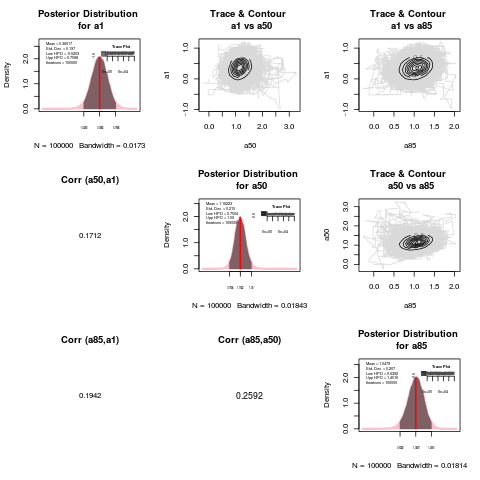
\includegraphics[scale=.5]{images/apost.pdf} 
            \caption{Posterior Distributions for $\alpha_1,\alpha_{50}$, and $\alpha_{85}$} \endmyfig 

\noindent
The chain also appears to have reached the correct distributions for the posterior of the other parameters
and hyper parameters. Here we will not discuss the plots in detail, but simply display them in Figure 2.
\beginmyfig 
\includegraphics[scale=.3]{images/hyperPost.pdf} 
            \caption{Posteriors and traceplots for parameters and hyper parameters}\endmyfig 

\noindent
The EPA is interested in the relationship between county level radon
measurements and county level uranium measurements. Figure 3 summarizes this
relationship. On the y-axis is the predicted log radon levels computed using
the estimated parameters. On the x-axis is the counties arranged in order of
predicted log radon levels. The red line is the predicted log radon level
for houses with basements, the blue line is the predicted log radon level
for houses without basements. The grey line is the measured log uranium level.
We see in general that as uranium levels increase, the radon levels increase. 
Moreover, we see that radon levels for houses with basements are higher than
those without. It is interesting to note, however, that it is not always the
case that counties with higher uranium levels have higher radon levels that
that of counties with lower uranium levels. This provides useful information
for the EPA as they can investigate why certain counties would have higher 
radon levels despite lower uranium levels. 

\beginmyfig \includegraphics[scale=.5]{images/ym.pdf}  
            \caption{The red and blue lines are the predicted log radon levels
            (log pCi/L) for house with basements and houses without basements
            for each county respectively. The grey line is the measured log
            soil uranium levels (log ppm) for each county.}\endmyfig 

%Of interest to the EPA was the relationship between county level radon measurements and 
%county level uranium measurements. This relationship can be observed by plotting the
%posterior means for each $\alpha_j$  against each corresponding $u_j$. The scatter plot
%with the fitted regression line is shown in Figure 3.
%\beginmyfig \includegraphics[scale=.5]{images/au.pdf}  
%            \caption{Estimated County Coefficients ($\alpha_j$) versus county
%            level log-uranium measures ($u_j$)}\endmyfig 


\section{Fitting The Bernoulli Model}
To extend these ideas to generalized linear models, I will
\beginmyfig 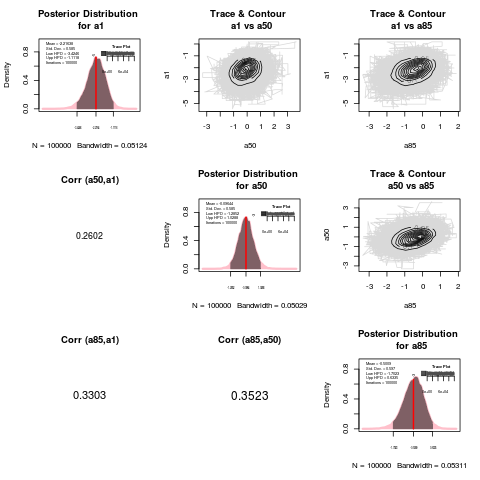
\includegraphics[scale=.5]{images/lapost.pdf} 
            \caption{Posterior Distributions for $\alpha_1,\alpha_{50}$, and $\alpha_{85}$} \endmyfig 

\beginmyfig 
\includegraphics[scale=.3]{images/lhyperPost.pdf} 
            \caption{Posteriors and traceplots for parameters and hyper parameters}\endmyfig 

\beginmyfig \includegraphics[scale=.5]{images/pm.pdf}  
            \caption{The figure above is the estimated probability of a house
            with a basement (red) and that of a house without a basement
            (blue), having radon levels above 4 for each county. The figure
            below is the measured log radon levels (log ppm) for each
            county.}\endmyfig 


\end{document}
